\input{../../cm10192}
%\input{../../cm10192-handout}

\author[Lecture D.7.]{Lecture D.7.: Java: Objects First
\\\begin{center}\input{../../copyright}\end{center}}

\lstset{language=Java}

\AtBeginSection[]
{
  \begin{frame}<beamer>
    \frametitle{Outline}
    \tableofcontents[currentsection,currentsubsection,hideothersubsections]
  \end{frame}
}

%\AtBeginSubsection[]
%{
%  \begin{frame}<beamer>
%    \frametitle{Outline}
%    \tableofcontents[currentsection,currentsubsection,hide]
%  \end{frame}
%}

\logo{\vbox{\hbox to 1.1cm{\hfil\includegraphics[width=1cm,keepaspectratio]{../../java}}}}

\def\gap{\qquad}
\let\ul\underline
\def\function#1{{\keytext{#1}}}



%------------------------------------------------------------------------

\begin{document}
\maketitle

\begin{frame}\frametitle{Resources}
\begin{itemize}
\item Objects First with Java. David J. Barnes and Michael K\"olling. Third edition
\item How to Think Like a Computer Scientist: Java. \url{http://www.greenteapress.com/thinkapjava/}
\item Big Java. Gay Horstman.
\item Thinking in Java. Bruce Eckel's \url{www.mindview.net/Books/TIJ4}
\item Sun Java Tutorials Series \url{http://java.sun.com/docs/books/tutorial/index.html}
\end{itemize}
\end{frame}

\begin{frame}\frametitle{Outline}
\tableofcontents[pausesections,hidesubsections]
\end{frame}

\section{Objections and Classes}

\begin{frame}
\frametitle{Fundamental Concepts}
\begin{itemize}
\item object
\item class
\item method
\item parameter
\item data type
\end{itemize}
\end{frame}

\subsection{Objects and Classes}

\begin{frame}
\frametitle{Objects and Classes}
\begin{itemize}
\item Objects
\begin{itemize}
\item represent ‘things’ from the real world, or from some problem domain 
(example: “the red car down there in the car park”)‏
\end{itemize}
\item Classes
\begin{itemize}
\item represent all objects of a kind (example: “car”)‏
\end{itemize}
\end{itemize}
\pause
Objects represent individual instantiations of the class. Object are \alert{instantiated}. 
\end{frame}

\begin{frame}
\frametitle{Exercise}
\begin{tabular}{ll}
TelephoneNumber & lord-of-the-rings \\
BankAccount & Diary\\
harry-potter-and-the-Philosopher-Stone  & myDiary\\
01225-38-5053 & marinaDeVos\\
Book & Lecturer\\
leonWatts & myAccount\\
\end{tabular}
\end{frame}

\begin{frame}
\frametitle{Objects and Classes}
\begin{center}
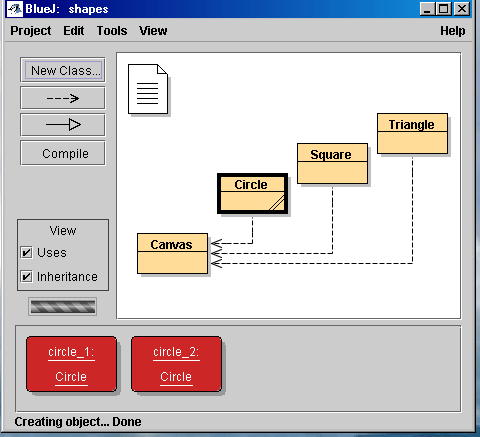
\includegraphics[height=5cm, keepaspectratio]{./figures/blueJ}
\end{center}
\end{frame}

\subsection{Methods}

\begin{frame}
\frametitle{Things we can do with objects I}
\begin{center}
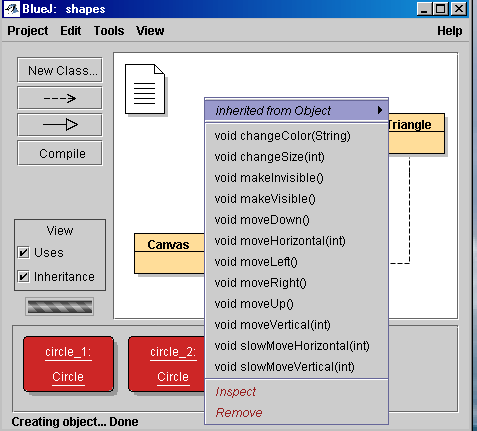
\includegraphics[height=5cm,keepaspectratio]{./figures/methods}
\end{center}
\end{frame}

\begin{frame}
\frametitle{Things we can do with objects II}
\begin{center}
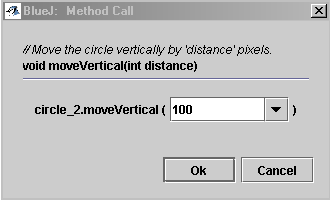
\includegraphics[height=5cm,keepaspectratio]{./figures/call}
\end{center}
\end{frame}




\begin{frame}
\frametitle{Methods and Parameters}
\begin{itemize}
\item Objects/classes have operations which can be invoked. They are called \alert{methods}
\item \lstinline!void moveHorizontal(int distance)! is called the \alert{signature} of the method 
\item The collection of methods of a class is referred to as the \alert{interface} of that class
\item methods may have \alert{parameters} to pass additional information needed to execute
\item Methods are \alert{called} or \alert{invoked}
\end{itemize}
\end{frame}

\begin{frame}
\frametitle{Exercise: BankAccount}
What are the methods should have BankAccount have?
\end{frame}

\begin{frame}
\frametitle{Abstract Data Types, Objects and Classes}
\begin{itemize}
\item In the Python lectures we discussed ADTs. They were implemented using nested functions. The outer function
returned a lambda function allowing you to access the inner functions.
\item A class is like this nested function
\item An object is the result from calling the function, i.e. the lambda.
\item Each time you call the outer function you will get a new lambda function and new internal data
\item The methods correspond to the inner functions.
\end{itemize}
\end{frame}

\begin{frame}
\frametitle{Data Types}
\begin{itemize}
\item Parameters have \alert{types}. A type defines what kinds of values a parameter can take.
\item In Java you have to specify the type. This was not the case for Python.
\item Defining a class defines a type
\item In Java, everything has a type.
\item Java is \alert{staticly typed language}
\item Examples of types: int, String, Circle, \ldots
\end{itemize}
\end{frame}

\subsection{Other Observations}

\begin{frame}
\frametitle{Other Observations}
\begin{itemize}
\item many \alert{instances} can be created from a single class
\item an object has \alert{attributes}: values stored in \alert{fields}. (The data you encapsulate)
\item the class defines what fields an object has, but each object stores its own set of values.
These set of values is called the \alert{state} of the object.
\end{itemize}
\end{frame}

\begin{frame}
\frametitle{State}
\begin{center}
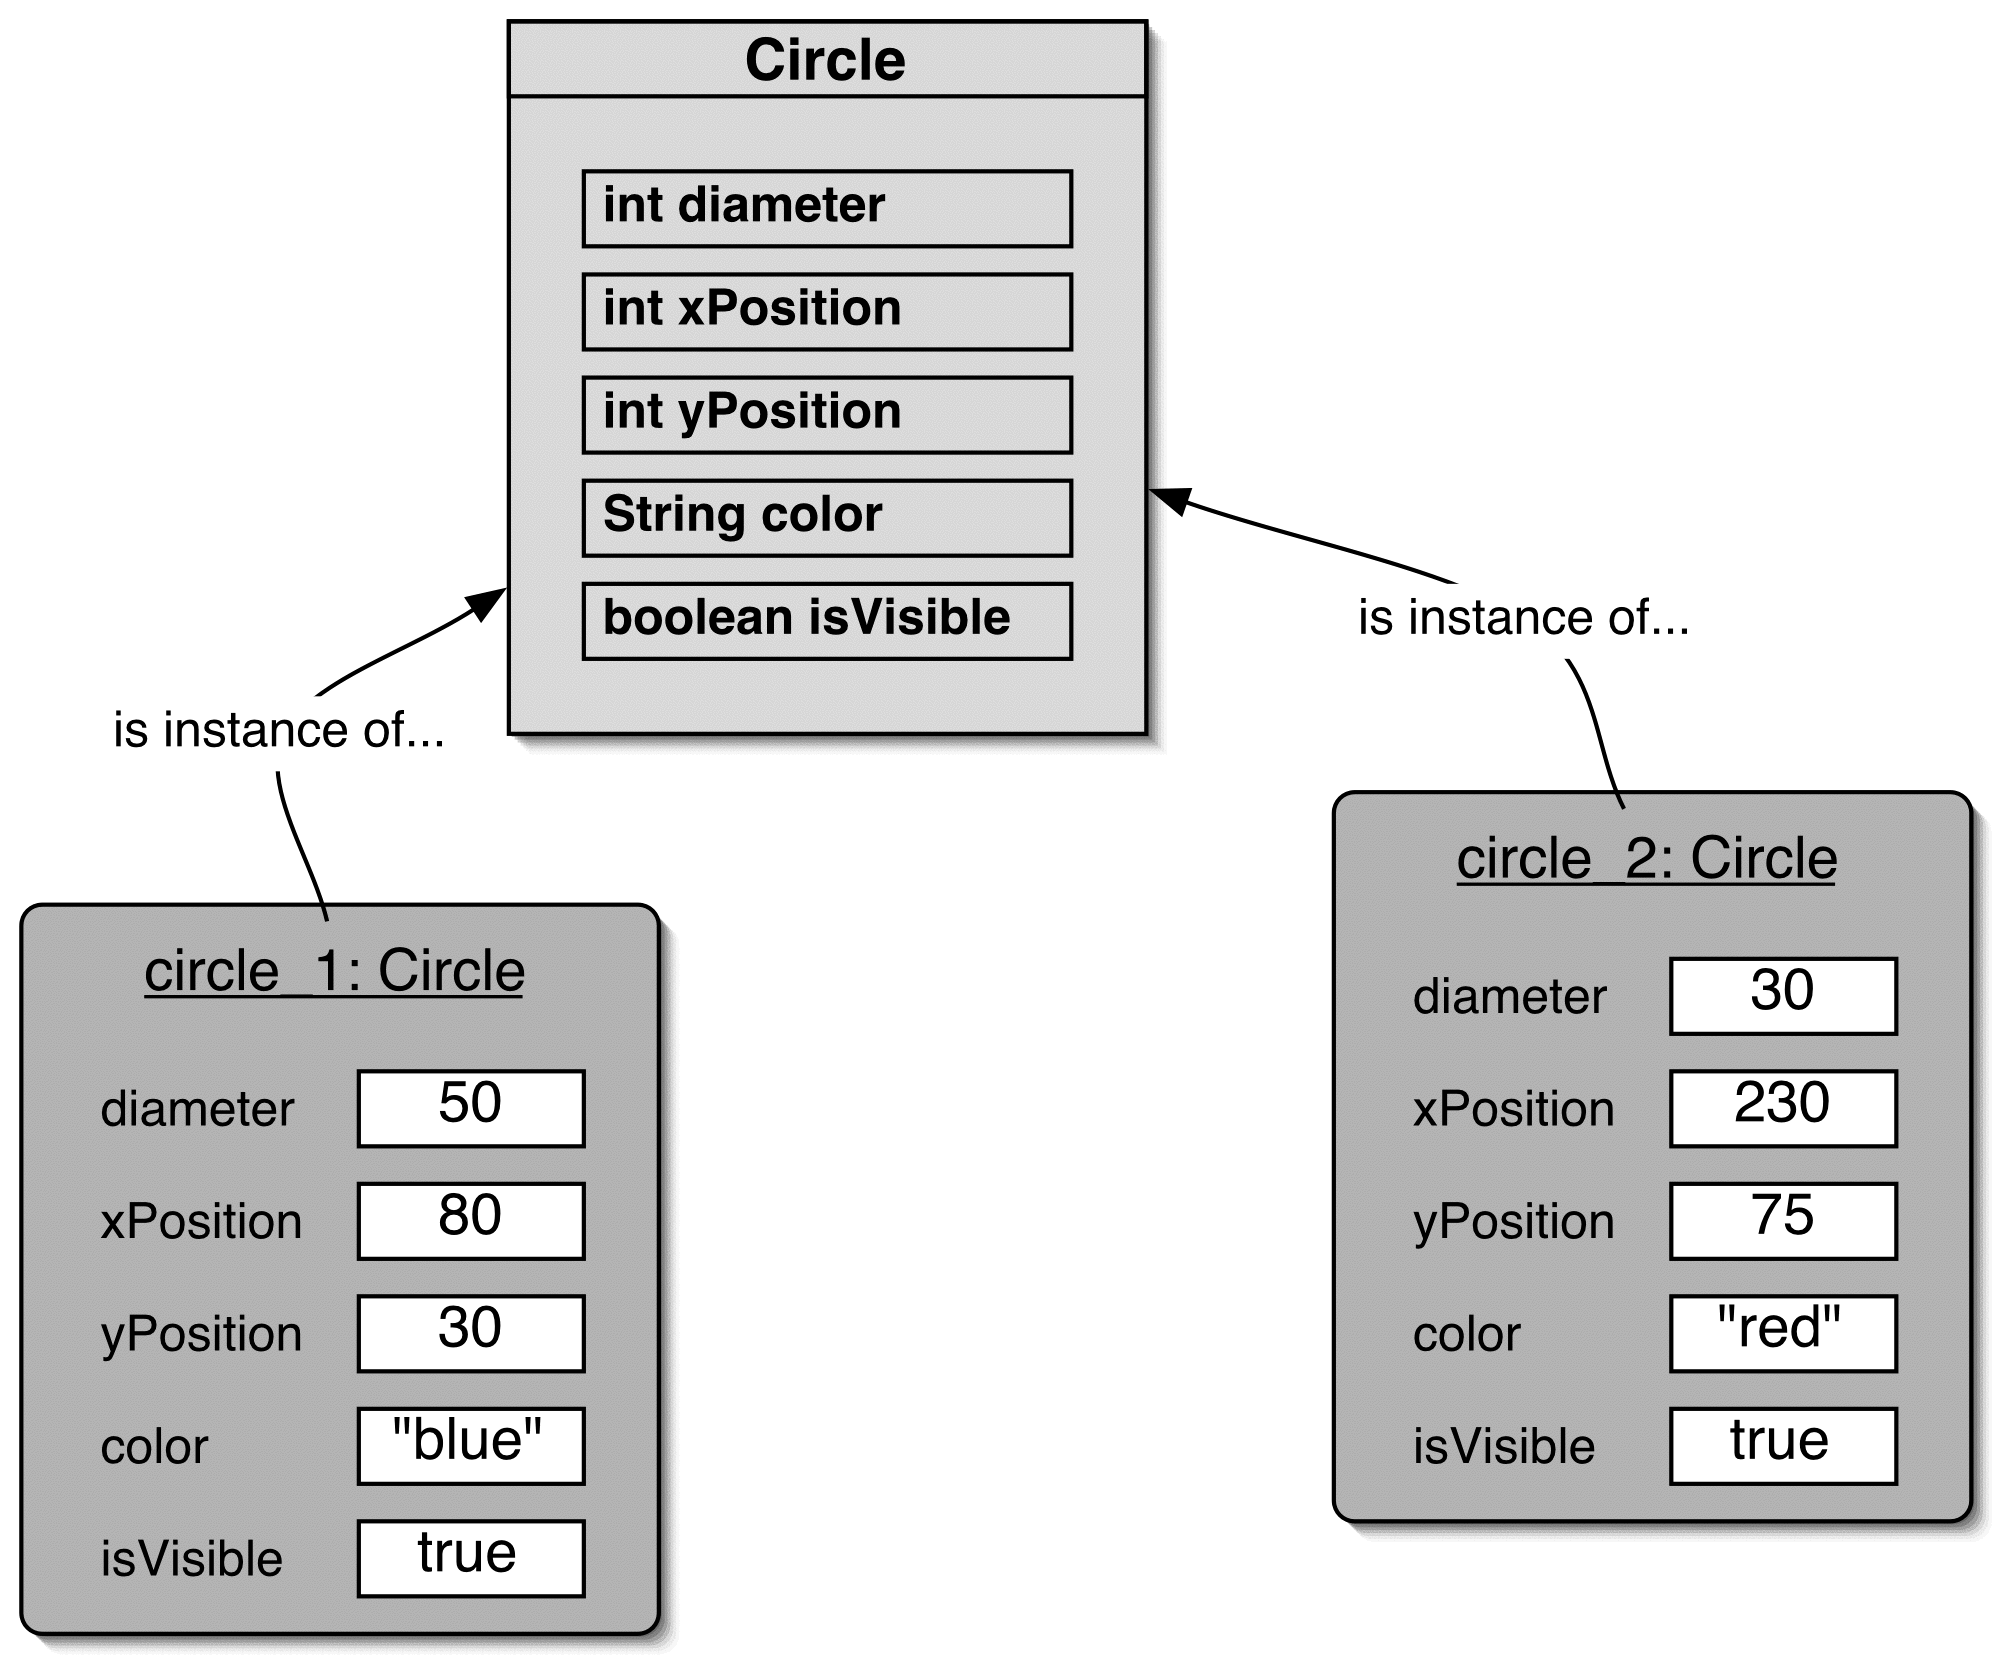
\includegraphics[height=5cm,keepaspectratio]{./figures/state}
\end{center}
\end{frame}




\begin{frame}
\frametitle{Object Interaction}
\begin{center}
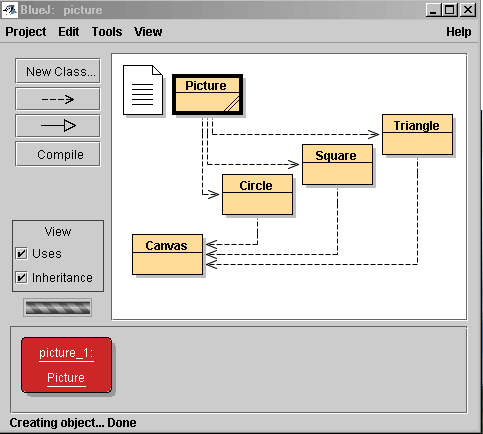
\includegraphics[height=5cm,keepaspectratio]{./figures/diagram}
\mbox{\hspace{0.1cm}}
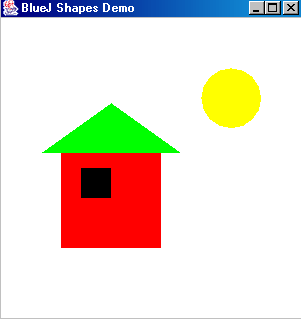
\includegraphics[height=5cm,keepaspectratio]{./figures/picture}
\end{center}
\end{frame}

\begin{frame}
\frametitle{Source Code}
\begin{itemize}
\item Each class has source code (Java code) associated with it that defines its details (fields and methods).
\item In other words, it determines the structure and the behavior of each of its instance.
\item This source code is compiled and interpreted by Java.
\end{itemize}
\end{frame}

\begin{frame}
\frametitle{Return Values}
\begin{itemize}
\item Methods may return a result via a \alert{return value}.
\item Example: \lstinline!String getName()‏!
This method returns a String.
\item Example: \lstinline!void changeName()‏!
\alert{Void} indicates that this method does not return anything
\end{itemize}
\end{frame}

\begin{frame}
\frametitle{Developing Java Programs}
\begin{itemize}
\item To learn to develop Java programs, one needs to learn how to write class definitions, including fields and methods, and how to put these classes together
\item During the rest of this unit we will deal with these issues in more detail
\end{itemize}
\end{frame}

\begin{frame}
\frametitle{Coding Conventions}
\begin{itemize}
\item Classes: Uppercase to start, merge words, consecutive words uppercase, nouns
E.g. Car, Number, BankAccount
\item Objects: Lowercase to start, merge words, consecutive words uppercase, nouns
E.g. myBlueCar, Rational
\item Methods: Lowercase to start, merge words, consecutive words uppercase, verbs
E.g. moveLocation, deposit
\end{itemize}
\end{frame}

\begin{frame}\frametitle{Glossary}
\rowcolors[]{1}{\lightrow}{\darkrow}
\begin{tabular}{|l|l|l|}
\hline
Object & Instance & State\\
\hline
Method & Invocation & Class\\
\hline
Source code & types & fields \\
\hline
Attribute & parameter & return value\\
\hline
\end{tabular}
\end{frame}


\section{Control Flow in Java}

\begin{frame}
\frametitle{Main concepts to be covered}
\begin{itemize}
\item fields
\item constructors
\item methods
\item parameters
\item assignment statements
\item conditional statements
\end{itemize}
\end{frame}

\subsection{Class Structure}

\begin{frame}
\frametitle{Ticket Machines – An External/User View}
Exploring the behaviour of a typical ticket machine.
\begin{itemize}
\item Use the naive-ticket-machine project.
\item Machines supply tickets of a fixed price.
\item How is that price determined?
\item How is ‘money’ entered into a machine?
\item How does a machine keep track of the money that is entered?
\item How is a ticket provided?
\end{itemize}
\end{frame}

\begin{frame}[fragile]
\frametitle{Resulting Fields: The State}
\codelist
\begin{lstlisting}[linewidth=5cm]
private int price = 500;
private int balance = 0;
private int total = 0;
\end{lstlisting}
\end{frame}

\begin{frame}[fragile]
\frametitle{Resulting Methods: The Interface}
\codelist
\begin{lstlisting}[linewidth=7cm]
public int getBalance()
public int getPrice()
public void insertMoney()
public void printTicket()
\end{lstlisting}
\end{frame}

\begin{frame}
\frametitle{Ticket Machines – An Internal/Programmer view}
\begin{itemize}
\item Interacting with an object gives us clues about its behavior.
\item Looking inside allows us to determine how that behavior is provided or implemented.
\begin{itemize}
\item Looking at the source code
\end{itemize}
\item All Java classes have a similar-looking internal view.
\end{itemize}
\end{frame}

\begin{frame}[fragile]
\frametitle{The Source Code}
\codelist
\codesmall
\begin{lstlisting}
/**
 * TicketMachine models a naive ticket machine that issues
 * flat-fare tickets.
 * The price of a ticket is specified via the constructor.
 * It is a naive machine in the sense that it trusts its users
 * to insert enough money before trying to print a ticket.
 * It also assumes that users enter sensible amounts.
 *
 * @author David J. Barnes and Michael Kolling
 * @version 2002.02.06
 */
public class TicketMachine
{
    // The price of a ticket from this machine.
    private int price;
    // The amount of money entered by a customer so far.
    private int balance;
    // The total amount of money collected by this machine.
    private int total;

    /**
     * Create a machine that issues tickets of the given price.
     * Note that the price must be greater than zero, and there
     * are no checks to ensure this.
     */
    public TicketMachine(int ticketCost)
    {
        price = ticketCost;
        balance = 0;
        total = 0;
    }

    /**
     * Return the price of a ticket.
     */
    public int getPrice()
    {
        return price;
    }
\end{lstlisting}
\end{frame}



\begin{frame}[fragile]
\frametitle{Basic class structure}
\begin{center}
\begin{tikzpicture}[scale=0.8]

\path[draw] node (outer) {\codelist \begin{lstlisting}[linewidth=5cm]
public class TicketMachine
{
    Inner part of 
    the class omitted.
}
\end{lstlisting}};

\path[draw] (outer)+(8,0) node[fill=\lightrow,rectangle,rounded corners=10pt] (otext1) {\begin{minipage}{4cm}
The outer wrapper of TicketMachine\end{minipage}};

\path[->,draw,color=diagram,line width=3pt] (otext1) -- (outer);


\path[draw] (outer)+(-0.5,-4) node (contents) {\codelist \begin{lstlisting}[linewidth=5cm]
public class ClassName
{
    Fields
    Constructors
    Methods
} 
\end{lstlisting}};



\path[draw] (contents)+(8,0) node[fill=\lightrow, rectangle,rounded corners=10pt] (otext2) {\begin{minipage}{4cm}The contents of a class\end{minipage}};


\path[->,draw,color=diagram,line width=3pt] (otext2) -- (contents);

\end{tikzpicture}
\end{center}
\end{frame}



\begin{frame}
\frametitle{Comments/Documentation}
\begin{itemize}
\item Comments make source code easier to read for humans. No effect on the functionality.
\item Three sorts:
\begin{itemize}
\item \lstinline!// comment!: single-line comments
\item \lstinline!/* comments */!: multiple-lines – more detail
\item \lstinline!/** */!: similar to previous, but used when documentation software is used.
\end{itemize}
\end{itemize}
\end{frame}

\begin{frame}[fragile]
\frametitle{Fields}
\begin{itemize}
\item \alert{Fields} store values for an object.
\item They are also known as \alert{instance variables}.
\item Fields define the \alert{state} of an object.
\item Fields have an associated \alert{type}.
\end{itemize}

\codelist
\codesmall
\begin{lstlisting}
public class TicketMachine
{
    private int price;
    private int balance;
    private int total;
 
    Constructor and methods omitted.
} 
\end{lstlisting}

\begin{center}
\begin{tikzpicture}[scale=0.8]
%\path[use as bounding box] (0,0) rectangle (4,4);

\draw node (private) {\alert{private int price}};

\path[draw]<2-> (private)+(-3,1.3) node (vis) {visibility modifier}; 
\path[draw]<3-> (private)+(0.2,1.3) node (type) {type};
\path[draw]<4-> (private)+(2,1.3) node (name) {name};

\path[coordinate]<2-> (vis)+(0,-1.35) coordinate(a1);
\path[coordinate]<4-> (name)+(0.4,-1.35) coordinate(a2);
\path[coordinate]<3-> (private.north)+(0.2,0) coordinate(a3);


\path[->,draw,color=diagram,line width=1pt]<2-> (vis) .. controls (a1) .. (private.west);
\path[->,draw,color=diagram,line width=1pt]<3-> (type) -- (a3); 
\path[->,draw,color=diagram,line width=1pt]<4-> (name.south)+(0.4,0) .. controls (a2) .. (private.east);

\end{tikzpicture}
\end{center}
\end{frame}


\subsection{Constructors}

\begin{frame}[fragile]
\frametitle{Constructors}
\begin{itemize}
\item Constructors create and initialize an object.
\item Then assign the necessary memory to the created object
\item They have the same name as their class.
\item They store initial values into the fields.
\item They often receive external parameter values for this.
\item They Passing data via parameters
\end{itemize}
\pause
\codelist
\begin{lstlisting}[linewidth=7cm]
public TicketMachine(int ticketCost)‏
{
    price = ticketCost;
    balance = 0;
    total = 0;
} 
\end{lstlisting}
\end{frame}

\begin{frame}[fragile]
\frametitle{Creating Objects}
\begin{itemize}
\item Constructors are used to create and initialise a new object
\codelist
\begin{lstlisting}[linewidth=8cm]
TicketMachine machine = new TicketMachine(500);
\end{lstlisting}
\item This creates a new TicketMachine object and stores it a variable named machine which is
of type TicketMachine.
\end{itemize}
\end{frame}

\begin{frame}
\frametitle{Object Diagram}

\begin{tikzpicture}[scale=0.8]
\path[draw] node (call) {\alert{\begin{minipage}{5cm}TicketMachine machine =\\ \hspace{1cm} new TicketMachine(500)\end{minipage}}};


\path[draw] (call.east)+(3,0) node[fill=\darkrow,rectangle,rounded corners=10pt,text centered,minimum height=6cm,minimum width=4cm] (state) {};

\path[draw] (state.north)+(0,-1) node (statec) {\begin{minipage}{4cm}\begin{center}\underline{machine:}\\\underline{TicketMachine} \end{center}\end{minipage}};

\path[draw] (statec.south)+(-1.5,-0.8) node[minimum width=1cm] (price) {price};
\path[draw] (price)+(0,-0.8) node[minimum height=1cm,minimum width=1cm] (balance) {balance};
\path[draw] (balance)+(0,-0.8) node[minimum height=1cm,minimum width=1cm] (total) {total};

\path[draw] (price)+(3,0) node[fill=white,rectangle,minimum height=0.5cm,minimum width=1cm] (p) {500};
\path[draw] (balance)+(3,0) node[fill=white,rectangle,minimum height=0.5cm,minimum width=1cm] (b) {0};
\path[draw] (total)+(3,0) node[fill=white,rectangle,minimum height=0.5cm,minimum width=1cm] (t) {0};

\path[draw] (total.south)+(1.5,-1.4) node[fill=\lightrow,rectangle,minimum height=2cm,minimum width=3.5cm] (con) {};

\path[draw] (con.north)+(0.4,-0.7) node (cc) {\begin{minipage}{3cm}
\small{TicketMachine}\\ \small{(constructor)} \end{minipage}};

\path[draw] (total)+(0.5,-2.4) node (cost) {ticketCost};
\path[draw] (cost)+(2.3,0) node[fill=white,rectangle,minimum height=0.5cm,minimum width=1cm] (cc) {500};

\path[coordinate] (cc.west)+(0,0.2) coordinate(a1);
\path[coordinate] (cc.west)+(-10,0.5) coordinate(a2);
\path[coordinate] (total.east)+(6,0) coordinate(a3);

\path[->,draw,color=diagram,line width=2pt] (call.south) .. controls(a2) .. (a1);
\path[->,draw,color=diagram,line width=2pt] (cc.north) .. controls(a3) .. (p.south);


\end{tikzpicture}
\end{frame}


\subsection{Methods - Parameters}

\begin{frame}[fragile]
\frametitle{Parameters}
\begin{itemize}
\item Just like in Python
\item Parameter names inside a constructor or method are referred to as \alert{Formal Parameters}
\item Parameter values provided from the outside are referred to as \alert{Actual Parameters}.
\item In the constructor \lstinline!TicketMachine(int ticketCost)! ticketCost is a 
formal parameter. When the constructor is called, \lstinline!TicketMachine(500)!, 500 is an actual parameter.
\end{itemize}
\end{frame}

\begin{frame}
\frametitle{Space}
\begin{itemize}
\item The ticketCost box  in the object representation is only created when the constructor is executed.
\item Extra temporarily storage is provided to store a value for ticketCost. This is called the constructor space or method space.
\item Values can only be used during the execution. 
\end{itemize}
\end{frame}

\begin{frame}
\frametitle{Scope and Lifetime}
\begin{itemize}
\item The \alert{scope} of a variable/parameter defines the section of the code from where it can be accessed.
\item For instance variables this is the entire class.
\item For parameters, this is the constructor or method that declares it. 
\item Trick: find the enclosing {}, this is the scope. 
\item The \alert{lifetime} of a variable/parameter describes how long the variable continues to exist before it is destroyed.
\item Concept the same as in Python. 
\end{itemize}
\end{frame}

\begin{frame}[fragile]
\frametitle{Assignment}
\begin{itemize}
\item Similar to Python
\item Values are stored into fields (and other variables) via \alert{assignment} statements:
\begin{itemize}
\item \lstinline!variable = expression;!
\item \lstinline!price = ticketCost;!
\end{itemize}
\item Both sides of the assignment should have the same type, e.g. int, double, String, TicketMachine, ...
\item A variable stores a single value, so any previous value is lost.
\end{itemize}
\end{frame}

\begin{frame}[fragile]
\frametitle{Accessor Methods I}
\begin{itemize}
\item Methods implement the behaviour of objects.
\item Accessors provide information about an object.
\item Methods have a structure consisting of a header and a body.
\item The header defines the \alert{method’s signature}.    \\
\lstinline!public int getPrice()‏!
\item The body encloses the method’s statements.
\end{itemize}
\end{frame}

\begin{frame}[fragile]
\frametitle{Accessor Methods II}
\begin{tikzpicture}[scale=0.8]
\path[draw] node (code) {\codelist
\begin{lstlisting}[linewidth=5cm]
public int getPrice()‏
{
    return price;
} 
\end{lstlisting}};

\path[draw]<2-> (code.north)+(-3,1.5) node[minimum height=1cm] (vis) {visibility modifier};
\path[draw]<3-> (vis)+(3.5,0.05) node[minimum height=1cm] (ret) {return value};
\path[draw]<4-> (ret)+(3,0) node[minimum height=1cm] (met) {method name}; 
\path[draw]<5-> (met)+(4,-0.05) node (par) {parameter list (empty)};

\path[draw]<6-> (code.east)+(3.5,0) node (rs) {return statement};

\path[draw]<7-> (code.south)+(1,-1.5) node (sf) {start end finish of the method (block)};

\path[coordinate] (code.north)+(-2,-0.1) coordinate(p);
\path[coordinate] (code.north)+(-1,-0.1) coordinate(r);
\path[coordinate] (code.north)+(1.5,-0.1) coordinate(m);
\path[coordinate] (code.north)+(2,-0.1) coordinate(pr);

\path[coordinate] (code.east)+(-1,0) coordinate(rv);

\path[coordinate] (code.west)+(-1,1) coordinate(b1);
\path[coordinate] (code.west)+(-1,-0.6) coordinate(b2);

\path[coordinate]<7-> (sf.west)+(-1,0) coordinate(b5);

\path[coordinate]<7-> (b5)+(0,3.15) coordinate(b4);
\path[coordinate]<7-> (b4)+(1.3,0) coordinate(b3);
\path[coordinate]<7-> (b5)+(0,2.15) coordinate(b2);
\path[coordinate]<7-> (b2)+(1.3,0) coordinate(b1);

\path[->,draw,color=diagram,line width=1pt]<2-> (vis) -- (p);
\path[->,draw,color=diagram,line width=1pt]<3-> (ret) -- (r);
\path[->,draw,color=diagram,line width=1pt]<4-> (met) -- (m);
\path[->,draw,color=diagram,line width=1pt]<5-> (par) -- (pr);
\path[->,draw,color=diagram,line width=1pt]<6-> (rs) -- (rv);

\path[->,draw,color=diagram,line width=1pt]<7-> (sf.west) -- (b5) -- (b4) -- (b3);
\path[->,draw,color=diagram,line width=1pt]<7-> (sf.west) -- (b5) -- (b2) -- (b1);


\end{tikzpicture}
\end{frame}



\begin{frame}
\frametitle{Mutator Methods}
\begin{itemize}
\item Have a similar method structure: header and body.
\item Used to \alert{mutate} (i.e., change) an object’s state.
\item Achieved through changing the value of one or more fields.
\begin{itemize}
\item Typically contain assignment statements.
\item Typically receive parameters.
\end{itemize}
\end{itemize}
\end{frame}

\begin{frame}[fragile]
\frametitle{Mutator methods}
\begin{tikzpicture}[scale=0.8]
\path[draw] node (code) {\codelist
\begin{lstlisting}[linewidth=7.3cm]
public void insertMoney(int amount)‏
{
    balance += amount;
} 
\end{lstlisting}};

\path[draw]<2-> (code.north)+(-3,1.5) node[minimum height=1cm] (vis) {visibility modifier};
\path[draw]<3-> (vis)+(3.5,0.05) node[minimum height=1cm] (ret) {return value};
\path[draw]<4-> (ret)+(3,0) node[minimum height=1cm] (met) {method name}; 
\path[draw]<5-> (met)+(3,-0.05) node (par) {parameter};

\path[draw]<6-> (code.east)+(2.5,0) node (rs) {assignment};

\path[draw]<7-> (code.south)+(2,-1.5) node (sf) {field being changed.};

\path[coordinate] (code.north)+(-4,-0.1) coordinate(p);
\path[coordinate] (code.north)+(-2,-0.1) coordinate(r);
\path[coordinate] (code.north)+(-1,-0.1) coordinate(m);
\path[coordinate] (code.north)+(2,-0.1) coordinate(pr);

\path[coordinate] (code.east)+(-4,0) coordinate(rv);

\path[coordinate] (code.west)+(-1,1) coordinate(b1);
\path[coordinate] (code.west)+(-1,-0.6) coordinate(b2);


\path[coordinate] (sf.west)+(-2,0) coordinate(b5);

\path[coordinate] (b5)+(0,2.4) coordinate(b4);

\path[->,draw,color=diagram,line width=1pt]<2-> (vis) -- (p);
\path[->,draw,color=diagram,line width=1pt]<3-> (ret) -- (r);
\path[->,draw,color=diagram,line width=1pt]<4-> (met) -- (m);
\path[->,draw,color=diagram,line width=1pt]<5-> (par) -- (pr);
\path[->,draw,color=diagram,line width=1pt]<6-> (rs) -- (rv);

\path[->,draw,color=diagram,line width=1pt]<7-> (sf.west) .. controls(b5) .. (b4);



\end{tikzpicture}
\end{frame}




\begin{frame}
\frametitle{Abstract Data Types}
\begin{itemize}
\item Classes define types
\item Can be used as parameter, field and return types
\item The internal is hidden from the user
\begin{itemize}
\item No direct access to fields (unless special reason)‏
\item Access to state via accessor and mutator methods
\end{itemize}
\item User does not need to know how the class is implemented to use/instantiate it
\item The usage of a class is defined by its methods
\end{itemize}
\end{frame}

\begin{frame}[fragile]
\frametitle{Printing from methods}
\codelist
\begin{lstlisting}
public void printTicket()‏
{
    // Simulate the printing of a ticket.
    System.out.println("##################");
    System.out.println("# The BlueJ Line");
    System.out.println("# Ticket");
    System.out.println("# " + price + " cents.");
    System.out.println("##################");
    System.out.println();
 
    // Update the total collected with the balance.
    total += balance;
    // Clear the balance.
    balance = 0;
} 
\end{lstlisting}
\end{frame}

\begin{frame}
\frametitle{Output}
\begin{center}
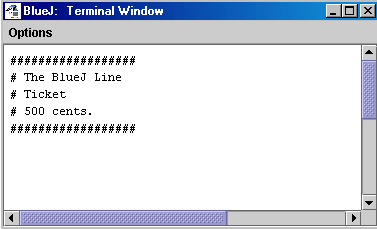
\includegraphics[height=5cm, keepaspectratio]{./figures/ticketOut}
\end{center}
\end{frame}

\subsection{Making Choices}

\begin{frame}
\frametitle{Reflecting on the ticket machines}
\begin{itemize}
\item Their behaviour is inadequate in several ways:
\begin{itemize}
\item No checks on the amounts entered.
\item No refunds.
\item No checks for a sensible initialization.
\end{itemize}
\item How can we do better?
\begin{itemize}
\item We need more sophisticated behaviour.
\end{itemize}
\end{itemize}
\end{frame}

\begin{frame}[fragile]
\frametitle{Making choices}
\codelist
\begin{lstlisting}
public void insertMoney(int amount)‏
{
    if(amount > 0) {
        balance += amount;
    }
    else {
        System.out.println("Use a positive amount: " +
                           amount);
    }
}
\end{lstlisting}
\end{frame} 


\begin{frame}[fragile]
\frametitle{Making choices}

\begin{tikzpicture}[scale=0.8]
\path[draw] node (code) {\codelist
\begin{lstlisting}
if(perform some test) {
    Do the statements here if the test gave a true result
}
else {
    Do the statements here if the test gave a false result
} 
\end{lstlisting}};

\path[draw]<2-> (code.north)+(-5,1) node (if) {‘if’ keyword};
\path[draw]<3-> (code.north)+(0,2) node (bool) {\begin{minipage}{7cm}boolean condition to be tested\\- gives a true or false result \end{minipage}};
\path[draw]<4-> (code.north)+(3,1) node (true) {actions if condition is true};
\path[draw]<5-> (code.south)+(-5,-1) node (else) {‘else’ keyword}; 
\path[draw]<6-> (code.south)+(3,-1) node (false) {actions if condition is false};

\path[coordinate] (code.north)+(-6.5,-0.1) coordinate(a);
\path[coordinate] (code.north)+(-4,-0.2) coordinate(b);
\path[coordinate] (code.north)+(0,-0.6) coordinate(c);
\path[coordinate] (code.south)+(-6.5,1.9) coordinate(d);
\path[coordinate] (code.south)+(0,1.6) coordinate(e);

\path[->,draw,color=diagram,line width=1pt]<2-> (if) -- (a);
\path[->,draw,color=diagram,line width=1pt]<3-> (bool.south)+(-2,0) -- (b);
\path[->,draw,color=diagram,line width=1pt]<4-> (true) -- (c);
\path[->,draw,color=diagram,line width=1pt]<5-> (else) -- (d);
\path[->,draw,color=diagram,line width=1pt]<6-> (false) -- (e);

\end{tikzpicture}
\end{frame}



\begin{frame}[fragile]
\frametitle{Boolean Tests}
\begin{itemize}
\item{$==$} : equality
\item{$>$} : greater than
\item{$<$} : less than
\item{$<=$} : less or equal than
\item{$>=$} : greater or equal than
\item{$!=$} : not equal
\end{itemize}
\end{frame}

\begin{frame}
\frametitle{Local variables}
\begin{itemize}
\item Fields are one sort of variable.
\begin{itemize}
\item They store values through the life of an object.
\item They are accessible throughout the class.
\item A bit like global variables in Python
\end{itemize}
\item Methods can include shorter-lived variables.
\begin{itemize}
\item They exist only as long as the method is being executed.
\item They are only accessible from within the method.
\item Like function variables in Python
\end{itemize}
\end{itemize}
\end{frame}

\begin{frame}[fragile]
\frametitle{Local variables} % tikz

\begin{tikzpicture}[scale=0.8]
\path[draw] node (code) {
\codelist
\begin{lstlisting}[linewidth=5cm]
public int refundBalance()‏
{
    int amountToRefund;
    amountToRefund = balance;
    balance = 0;
    return amountToRefund;
} 
\end{lstlisting}};

\path[draw]<2-> (code.east)+(1,-3) node (lv) {local variable};
\path[draw]<3-> (code.west)+(-1,-3) node (vm) {\alert{no visibility modifier}};

\path[coordinate] (code.east)+(-1.2,0.6) coordinate(a);
\path[coordinate] (code.west)+(0.7,0.6) coordinate(b);
\path[coordinate] (code.east)+(1,0) coordinate(c);
\path[coordinate] (code.east)+(-10,0) coordinate(d);

\path[->,draw,color=diagram,line width=1pt]<2-> (lv) .. controls(c) .. (a);
\path[->,draw,color=diagram,line width=1.5pt]<3-> (vm) .. controls(d) .. (b);

\end{tikzpicture}
\end{frame}



\begin{frame}
\frametitle{Review}
\begin{itemize}
\item Class bodies contain fields, constructors and methods.
\item Fields store values that determine an object’s state.
\item Constructors initialize objects.
\item Methods implement the behaviour of objects.
\item Constructors are methods which do not return anything. 
\end{itemize}
\end{frame}

\begin{frame}
\frametitle{Review}
\begin{itemize}
\item Fields, parameters and local variables are all variables.
\item Fields persist for the lifetime of an object.
\item Parameters are used to receive values into a constructor or method.
\item Local variables are used for short-lived temporary storage. 
\item Objects can make decisions via conditional (if) statements.
\item A true or false test allows one of two alternative courses of actions to be taken.
\end{itemize}
\end{frame}

\begin{frame}
\frametitle{Coding Convention}
\begin{itemize}
\item If statement
\begin{itemize}
\item Always use \{ , even if there is only one statement
\item In case there is an else statement, start on a new line and use \{
\end{itemize}
\item Indentation
\begin{itemize}
\item Always indent your code, even if your text editor does not do it automatically
\end{itemize}
\item Document your code, the sooner the better. 
\end{itemize}
\end{frame}


\begin{frame}{Glossary}
\rowcolors[]{1}{\lightrow}{\darkrow}
\begin{tabular}{|l|l|l|}
\hline
Terms & Instance variables & Local variables\\
\hline
Parameters & Formal Parameters & Actual Parameters\\
\hline 
Scope & Lifetime & Assignment\\
\hline
Constructors & Methods & \\
\hline
If-statement & Object diagram & \\
\hline
\end{tabular}
\end{frame}

\section{Object Interaction}

\begin{frame}
\frametitle{Main concepts to be covered}
\begin{itemize}
\item Abstraction
\item Modularization
\item Class and Object Diagrams
\item Call-by-reference and Call-by-value
\item Overloading
\item Internal and External method calls
\item this keyword
\item Debugging
\end{itemize}
\end{frame}

\subsection{Abstraction \& Modularisation}

\begin{frame}
\frametitle{A digital clock}
\begin{center}
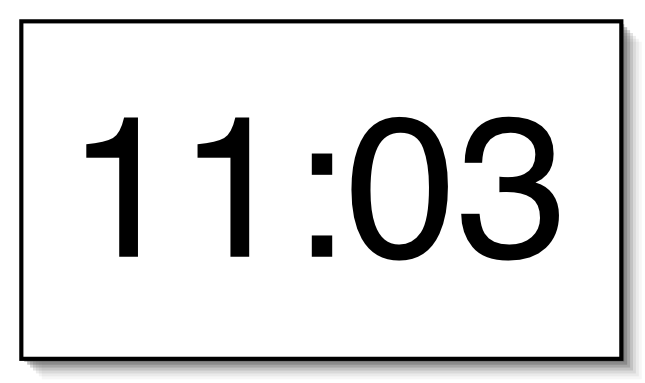
\includegraphics[height=5cm,keepaspectratio]{./figures/clock}
\end{center}
\end{frame}

\begin{frame}
\frametitle{Abstraction and modularization}
\begin{itemize}
\item \alert{Abstraction} is the ability to ignore details of parts to focus attention on a higher level of a problem. 
\item \alert{Modularization} is the process of dividing a whole into well-defined parts, which can be built and examined separately, and which interact in well-defined ways. 
\end{itemize}
\end{frame}

\begin{frame}
\frametitle{Modularizing the clock display}
\begin{tabular}{lll}
\begin{minipage}{3cm}
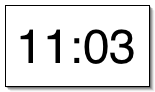
\includegraphics[height=1cm,keepaspectratio]{./figures/cl1} \end{minipage} & \mbox{}\hspace{1cm} & One four-digit display?\\
\mbox{}\\
\begin{minipage}{3cm}
Or two two-digit displays
\end{minipage}& & \begin{minipage}{3cm}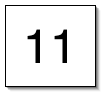
\includegraphics[height=1cm,keepaspectratio]{./figures/cl2}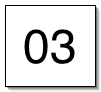
\includegraphics[height=1cm,keepaspectratio]{./figures/cl3}\end{minipage}
\end{tabular}
\end{frame}


\begin{frame}[fragile]
\frametitle{Implementation: NumberDisplay}
\codelist
\begin{lstlisting}[linewidth=6cm]
public class NumberDisplay
{
    private int limit;
    private int value;

    Constructor and
    methods omitted.
}
\end{lstlisting}
\end{frame}

\begin{frame}[fragile]
\frametitle{Implementation: ClockDisplay}
\codelist
\begin{lstlisting}[linewidth=7cm]
public class ClockDisplay
{
    private NumberDisplay hours;
    private NumberDisplay minutes;

    Constructor and
    methods omitted.
}
\end{lstlisting}
\end{frame}

\subsection{Diagrams}

\begin{frame}
\frametitle{Object diagram}
\begin{center}
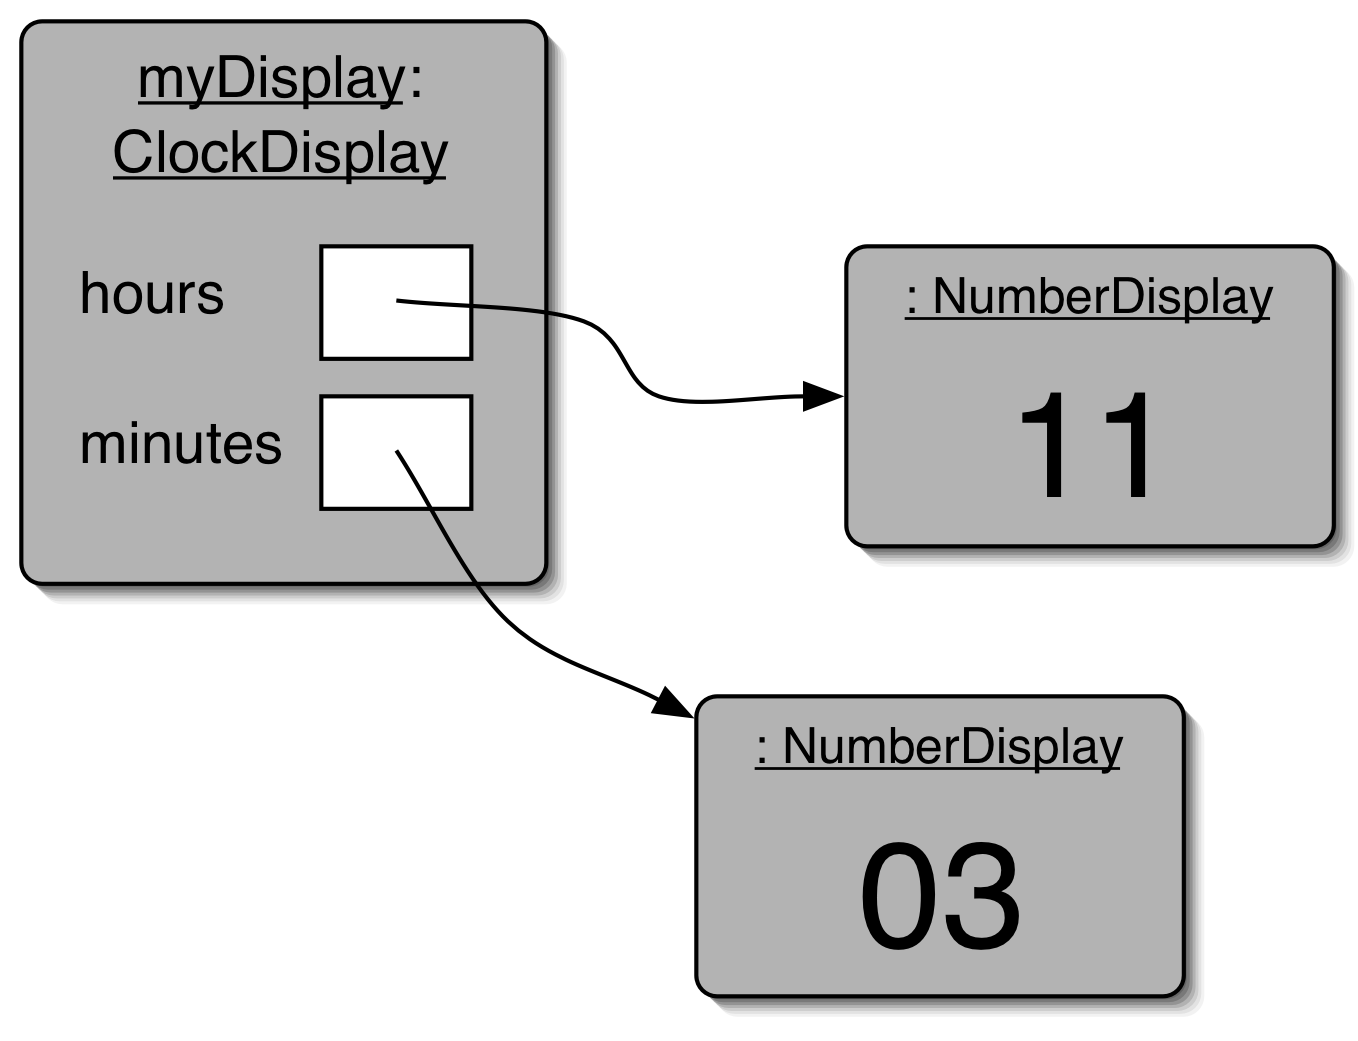
\includegraphics[height=5cm, keepaspectratio]{./figures/object}
\end{center}
\end{frame}

\begin{frame}
\frametitle{Class diagram}
\begin{center}
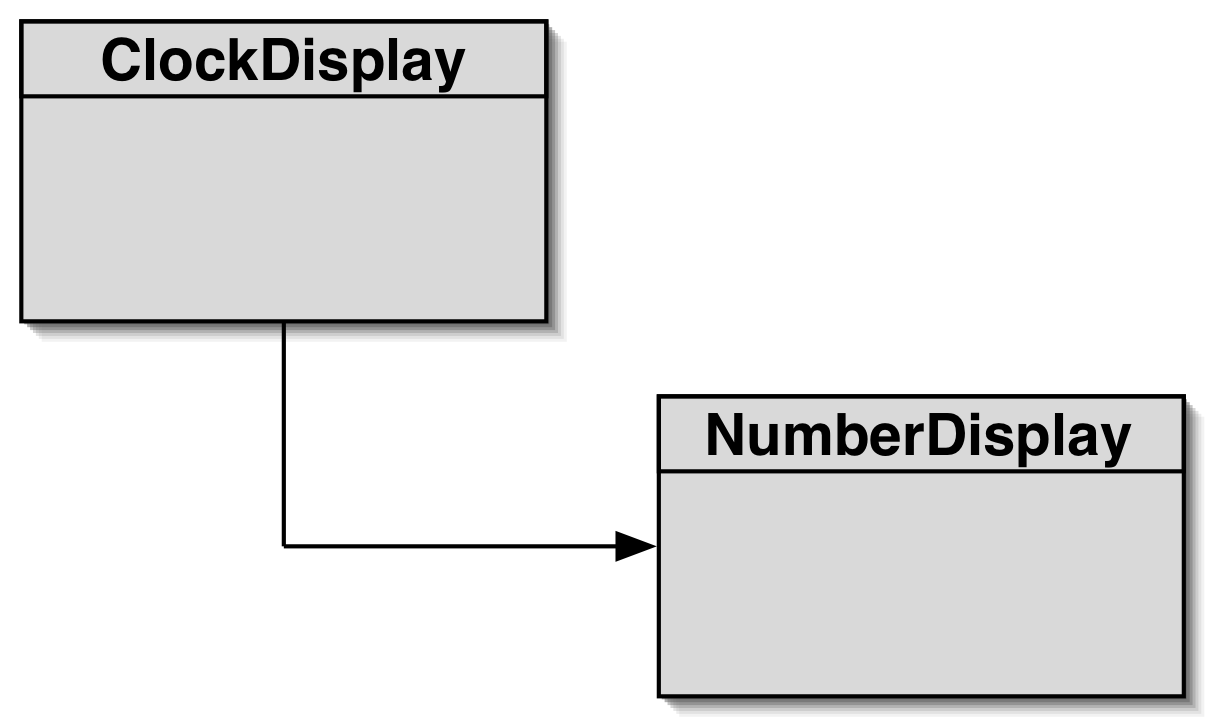
\includegraphics[height=5cm, keepaspectratio]{./figures/class}
\end{center}
\end{frame}

\begin{frame}
\frametitle{Diagrams}
\begin{itemize}
\item Class Diagrams
\begin{itemize}
\item Shows the classes of an application and the relationships between them
\item Gives information about the source code
\item Static view of the program
\end{itemize}
\item Object Diagrams
\begin{itemize}
\item Shows objects and their relationships at one moment in time during the execution of the program
\item Dynamic view of the program
\end{itemize}
\end{itemize}
\end{frame}



\subsection{Types}
\begin{frame}
\frametitle{Primitive types vs. object types}
\begin{itemize}
\item Java defines two very different kinds of type: primitive types and object types.
\item Primitive types are predefined by Java.
\item Object types originate from classes.
\item Variables and parameters store references to objects.
\item The primitive types are non-object types.
\item This is the reason why Java is not a completely object oriented languages
\end{itemize}
\end{frame}


\begin{frame}
\frametitle{Primitive types vs. object types} 
\begin{center}

\begin{tikzpicture}
\path[draw] node (el) {SomeObject obj;};
\path[draw] node[below of=el, draw=diagram,minimum width=1cm,minimum height=1cm,rectangle] (poin) {};
\path[draw] (poin)+(3,-1.2) node[draw=diagram, shade, ball color=\darkrow,minimum width=1.5cm,minimum height=1.5cm,rectangle,rounded corners=10pt] (mem) {};
\path[draw] (el)+(5,0) node (ty1) {Object Type};
\path[->,draw,color=diagram,line width=1.5pt] (poin.center) -- (mem);

\path[draw] (el)+(0,-4) node (el2) {int i;};
\path[draw] node[below of=el2, draw=diagram,minimum width=1cm,minimum height=1cm,rectangle] (val) {32};
\path[draw] (el2)+(5,0) node (ty2) {Primitive Type;};
\end{tikzpicture}
\end{center}
\end{frame}




\begin{frame}
\frametitle{Primitive types vs. object types} 

\begin{center}
\begin{tikzpicture}
\path[draw] node (ao) {SomeObject a;};
\path[draw] node[below of=ao, draw=diagram,minimum width=1cm,minimum height=1cm,rectangle] (poin1) {};
\path[draw] (poin1)+(3,-1.2) node[draw=diagram, shade, ball color=\darkrow,minimum width=1.5cm,minimum height=1.5cm,rectangle,rounded corners=10pt] (mem) {};
\path[draw] (ao)+(6,0) node (bo) {SomeObject b};
\path[draw] node[below of=bo, draw=diagram,minimum width=1cm,minimum height=1cm,rectangle] (poin2) {};

\path[draw] node[below of=mem] {\alert{a = b}};

\path[->,draw,color=diagram,line width=1.5pt] (poin1.center) -- (mem);
\path[->,draw,color=diagram,line width=1.5pt] (poin2.center) -- (mem);

\path[draw] (ao)+(0,-4) node (v1) {int a;};
\path[draw] node[below of=v1, draw=diagram,minimum width=1cm,minimum height=1cm,rectangle] (val1) {32};
\path[draw] (v1)+(6,0) node (v2) {int b;};
\path[draw] node[below of=v2, draw=diagram,minimum width=1cm,minimum height=1cm,rectangle] (val2) {32};
\end{tikzpicture}
\end{center}
\end{frame}



\subsection{Methods Again}

\begin{frame}
\frametitle{Call-by-reference and Call-by-value}
\begin{itemize}
\item There are two ways of passing arguments to methods in many programming languages: call-by-value and call-by-reference.
\item Call-by-value: A copy of the actual parameter is passed to the formal parameter of the called method. Any change made to the formal parameter will have no effect on the actual parameter.
\item Call-by-reference: the caller gives the called method the ability to directly access to the caller’s data and to modify that data if the called method so chooses.
\item Just like Python Java uses call-by-value
\item For objects, the value is a reference to memory (like in Python)
\end{itemize}
\end{frame}

\begin{frame}[fragile]
\frametitle{Source code: NumberDisplay}
\codelist
\begin{lstlisting}
public class NumberDisplay
{
    private int limit;
    private int value;

          public NumberDisplay(int rollOverLimit)‏
{
    limit = rollOverLimit;
    value = 0;
}
\end{lstlisting}
\end{frame}

\begin{frame}[fragile]
\frametitle{Source code: NumberDisplay}
\codelist
\begin{lstlisting}
public int getValue()‏
    {
        return value;
    }

public void setValue(int replacementValue)‏
    {
        if((replacementValue >= 0) && 
           (replacementValue < limit))‏
            value = replacementValue;
    }
\end{lstlisting}
\end{frame}


\begin{frame}
\frametitle{Logical Operators}
\begin{itemize}
\item \&\& : and, operands are tested, left to right, until conclusion can be reached 
\item $\mid \mid$ : or, operands are tested, left to right, until conclusion can be reached
\item ! : not
\item \& : and, both operands are tested
\item $\mid$ : or, both operands are tested
\end{itemize}
\end{frame}

\begin{frame}[fragile]
\frametitle{Source code: NumberDisplay}
\codelist
\begin{lstlisting}
public String getDisplayValue()‏
{
    if(value < 10)‏
        return "0" + value;
    else
        return "" + value;
}

public void increment()‏
    {
        value = (value + 1) % limit;
    }
\end{lstlisting}
\end{frame}

\begin{frame}
\frametitle{String Concatenation}
\begin{itemize}
\item Addition:
\begin{itemize}
\item 12 + 24
\end{itemize}
\item String Concatenation:
\begin{itemize}
\item ``Java'' + `` and Python'' $->$ ``Java and Python''
\item ``answer': '' + 42 $->$ ''answer: 42''
\end{itemize}
\end{itemize}
\end{frame}

\begin{frame}[fragile]
\frametitle{String toString() method}
\begin{itemize}
\item String toString() method: Java provides a way of transforming every Object into a String. 
\item To tailor this to your own preference write a method toString() returning a String representation of your class/object.
\codelist
\begin{lstlisting}
public String toString()‏
{
	return ``value: '' + value + `` with limit '' + limit;
}
\end{lstlisting}
\end{itemize}
\end{frame}

\begin{frame}
\frametitle{The Modulo Operator}
\begin{itemize}
\item \% : the modulo operator calculates the remainder of an integer division
\begin{itemize}
\item 27 \% 4 $->$ 3
\end{itemize}
\item Division in Java: if both arguments are integers, division will result in an integer.
\begin{itemize}
\item double res = 5 / 2 $->$ res = 2
\item double res = 5 / (2.0) or 5 / (2 * 1.0)    $->$ res = 2.5
\end{itemize}
\end{itemize}
\end{frame}

\begin{frame}[fragile]
\frametitle{Objects creating objects}
\codelist
\begin{lstlisting}
public class ClockDisplay
{
    private NumberDisplay hours;
    private NumberDisplay minutes;
    private String displayString; 
    
    public ClockDisplay()‏
    {
        hours = new NumberDisplay(24);
        minutes = new NumberDisplay(60);
        updateDisplay();
    }
}
\end{lstlisting}
\end{frame}

\begin{frame}
\frametitle{Objects creating objects}
\begin{enumerate}
\item new ClassName(parameter-list)‏
\begin{itemize}
\item It creates a new object of the named class
\begin{itemize}
\item here NumberDisplay
\item this involves creating sufficient memory to store the values of primitive instance variables and references to object instance variables.
\end{itemize}
\end{itemize}
\item It executes the constructor of that class
\end{enumerate}
\end{frame}

\begin{frame} 
\frametitle{ClockDisplay object diagram}
\begin{center}
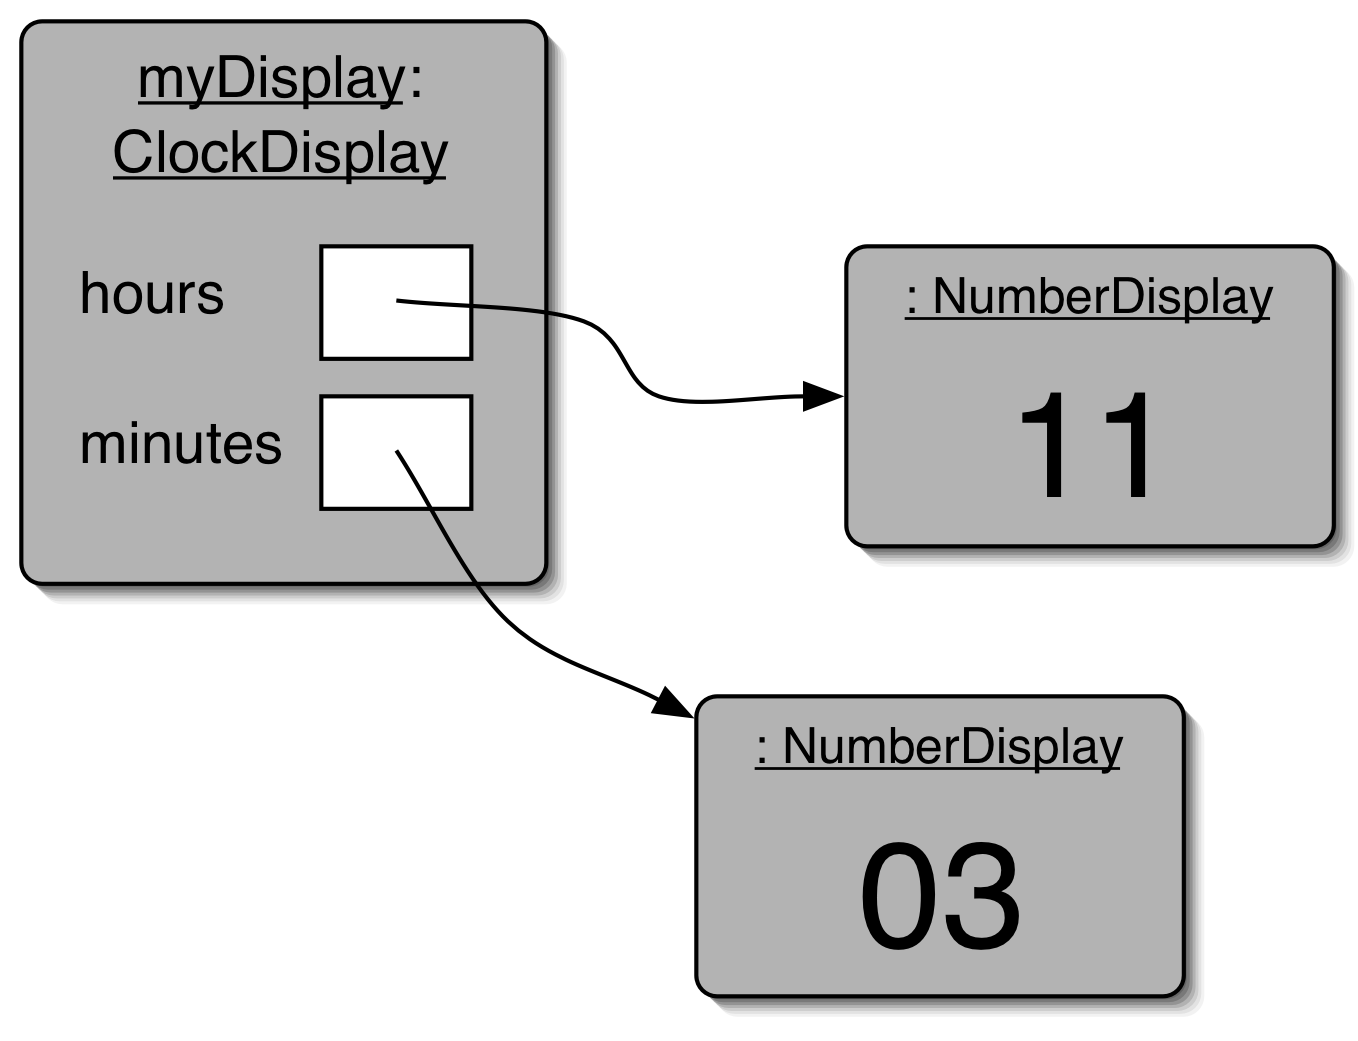
\includegraphics[height=5cm, keepaspectratio]{./figures/object}
\end{center}
\end{frame}

\begin{frame}
\frametitle{Method Overloading}
\begin{itemize}
\item Multiple Constructors of ClockDisplay:
\begin{itemize}
\item \lstinline!new Clockdisplay()‏!
\item \lstinline!new Clockdisplay(hour, minute)‏!
\end{itemize}
\item It is common for class definitions to contain alternative versions of constuctors or methods that provide various ways of achieving a particular task via their distinctive sets of parameters.
\item This is known as \alert{overloading}.
\end{itemize}
\end{frame}

\begin{frame}[fragile]
\frametitle{Method calling}
\codelist
\begin{lstlisting}
public void timeTick()‏
{
    minutes.increment();
    if(minutes.getValue() == 0) { 
        // it just rolled over!
        hours.increment();
    }
    updateDisplay();
}
\end{lstlisting}
\end{frame}

\begin{frame}[fragile]
\frametitle{Internal method}
\codelist
\begin{lstlisting}
/**
 * Update the internal string that
 * represents the display.
 */
private void updateDisplay()‏
{
    displayString = 
        hours.getDisplayValue() + ":" + 
        minutes.getDisplayValue();
}
\end{lstlisting}
\end{frame}

\begin{frame}[fragile]
\frametitle{Method calls}
\begin{itemize}
\item internal method calls
\codelist
\begin{lstlisting}[linewidth=6cm]
		updateDisplay();
		private void updateDisplay()‏
\end{lstlisting}
\begin{itemize}
\item \lstinline!methodName(parameter-list)!		
\end{itemize}
\item external method calls
\codelist
\begin{lstlisting}[linewidth=6cm]
		minutes.increment();
\end{lstlisting}
\begin{itemize}
\item object.methodName(parameter-list)‏
\end{itemize}
\end{itemize}
\end{frame}

\begin{frame}[fragile]
\frametitle{Public and Private Methods}
\begin{itemize}
\item Public methods:
\begin{itemize}
\item \lstinline!public void increment()‏!
\item can be called externally
\end{itemize}
\item Private methods
\begin{itemize}
\item \lstinline!private void updateDisplay()‏!
\item can only be called internally
\item used for auxiliary methods 
\end{itemize}
\end{itemize}
\end{frame}



\begin{frame}
\frametitle{The Mail System}
\begin{center}
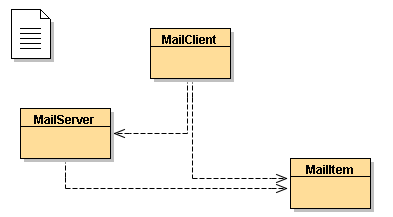
\includegraphics[height=5cm, keepaspectratio]{./figures/mailclass}
\end{center}
\end{frame}

\begin{frame}[fragile]
\frametitle{The this Keyword}
\codelist
\begin{lstlisting}
public class MailItem
{
	private String from;
	private String to;
	private String message;

  public MailItem(String from, String to, 
                  String message)‏
    {
        this.from = from;
        this.to = to;
        this.message = message;
    }
\end{lstlisting}
\end{frame}

\begin{frame}[fragile]
\frametitle{The this Keyword}
\begin{itemize}
\item \lstinline!this.from = from!
\begin{itemize}
\item \alert{name overloading}: the same name is used for two different entities: instance variable and formal parameter.
\item this is used to go out of the scope of the constructor to class level
\item \alert{\lstinline!this!} always refers to the current object.
\item can also used for methods
\item for internal methods calls and access to instance fields Java automatically inserts this:
\lstinline!updateDisplay -> this.updateDisplay!
\end{itemize}
\end{itemize}
\end{frame}


\begin{frame}{Glossary}
\rowcolors[]{1}{\lightrow}{\darkrow}
\begin{tabular}{|l|l|l|}
\hline
Abstraction & Modularisation & this\\
\hline
Call-by-value & Call-by-reference & Class diagram \\
\hline
Logical Operators & Modulo& Object diagram\\
\hline
\end{tabular}
\end{frame}

\section{Running Java Programs}

\subsection{Compiled/Interpreted Language}

\begin{frame}\frametitle{Interpreted Languages}
\newsavebox{\tikzbox}
\savebox{\tikzbox}{
\tikzstyle{block} = [draw=diagram, fill=example text.fg!20!bg, rectangle, 
    minimum height=3em, minimum width=6em]
\tikzstyle{pinstyle} = [pin edge={to-,thin,black}]


\begin{tikzpicture}[auto,>=latex']
\node [block] (controller) {Input};
\node [block, right of=controller, node distance=4cm] (system) {Interpreter};
\node [block, right of=system, node distance=4cm] (output) {Final Output};

\draw [-to,thick,snake=snake,segment amplitude=.4mm,draw=diagram,
         segment length=2mm,line after snake=1mm] (controller) -- node[name=u] {} (system);

\node [below of=u,text width=4cm,text centered, node distance=1.5cm] {\small{The interpreter reads in the source code ...}};

\draw [-to,thick,snake=snake,segment amplitude=.4mm, draw=diagram,
         segment length=2mm,line after snake=1mm] (system) -- node[name=w] {} (output);

\node [below of=w,text width=4cm,text centered, node distance=1.5cm] {\small{... and the result appears on the screen}};

\end{tikzpicture}
}
\begin{center}
\mode<presentation>{\resizebox{!}{0.3\textheight}{\usebox{\tikzbox}}}
\mode<article>{\resizebox{\textwidth}{!}{\usebox{\tikzbox}}}
\end{center}
\end{frame}

\begin{frame}\frametitle{Compiled Languages}
\savebox{\tikzbox}{
\tikzstyle{block} = [draw=diagram, fill=example text.fg!20!bg, rectangle, 
    minimum height=3em, minimum width=6em]
\tikzstyle{pinstyle} = [pin edge={to-,thin,black}]


\begin{tikzpicture}[auto,>=latex']
\node [block] (input) {Input};
\node [block, right of=input, node distance=4cm] (comp) {Compiler};
\node [block, right of=comp, node distance=4cm] (obj) {Object Code};
\node [block, right of=obj, node distance=4cm] (exe) {Executor};
\node [block, right of=exe, node distance=4cm] (output) {Output};

\draw [-to,thick,snake=snake,segment amplitude=.4mm,draw=diagram,
         segment length=2mm,line after snake=1mm] (input) -- node[name=u] {} (comp);

\node [below of=u,text width=4cm,text centered, node distance=1.5cm] {\small{The compiler reads in the source code ...}};

\draw [-to,thick,snake=snake,segment amplitude=.4mm, draw=diagram,
         segment length=2mm,line after snake=1mm] (comp) -- node[name=w] {} (obj);

\node [below of=w,text width=4cm,text centered, node distance=1.5cm] {\small{... and generate the object code ...}};

\draw [-to,thick,snake=snake,segment amplitude=.4mm, draw=diagram,
         segment length=2mm,line after snake=1mm] (obj) -- node[name=z] {} (exe);

\node [below of=z,text width=4cm,text centered, node distance=1.5cm] {\small{... you execute the code (one way or the other) ...}};

\draw [-to,thick,snake=snake,segment amplitude=.4mm, draw=diagram,
         segment length=2mm,line after snake=1mm] (exe) -- node[name=x] {} (output);

\node [below of=x,text width=4cm,text centered, node distance=1.5cm] {\small{... and the result appears on the screen}};

\end{tikzpicture}
}
\begin{center}
\mode<presentation>{\resizebox{\textwidth}{!}{\usebox{\tikzbox}}}
\mode<article>{\resizebox{\textwidth}{!}{\usebox{\tikzbox}}}
\end{center}
\end{frame}



\begin{frame}
\frametitle{The Programming Language Java}
\begin{itemize}
\item The Java language is both compiled and
interpreted.  
\item Instead of translating Java programs into a 
machine language, the Java compiler generates Java byte code for its \alert{Virtual Machine}
\begin{itemize}
\item Byte code is easy (and fast) to interpret, like machine language,
\item but it is also portable, like a high-level language.  
\end{itemize}
\item Thus, it is possible to compile a Java program on one machine,
transfer the byte code to another machine over a network,
and then interpret the byte code on the other machine.  
\item This ability is one of the advantages of Java over many other
high-level languages.
\end{itemize}
\end{frame}

\begin{frame}\frametitle{Java: Compile - Interpret}
\savebox{\tikzbox}{
\tikzstyle{block} = [draw=diagram, fill=example text.fg!20!bg, rectangle, 
    minimum height=3em, minimum width=6em]
\tikzstyle{block2} = [draw=diagram, fill=example text.fg!20!bg, ellipse, 
    minimum height=3em, minimum width=6em]
\tikzstyle{pinstyle} = [pin edge={to-,thin,black}]


\begin{tikzpicture}[auto,>=latex']
\node [block] (input) {Input};
\node [block2, right of=input, node distance=4cm] (comp) {Compiler};
\node [block, right of=comp, node distance=4cm] (obj) {Virtual Machine Code};
\node [block2, right of=obj, node distance=4cm] (exe) {Interpreter};
\node [block, right of=exe, node distance=4cm] (output) {Output};

\draw [-to,thick,snake=snake,segment amplitude=.4mm,draw=diagram,
         segment length=2mm,line after snake=1mm] (input) -- node[name=u] {} (comp);

\node [below of=u,text width=4cm,text centered, node distance=1.5cm] {\small{The compiler reads in the source code ...}};

\draw [-to,thick,snake=snake,segment amplitude=.4mm, draw=diagram,
         segment length=2mm,line after snake=1mm] (comp) -- node[name=w] {} (obj);

\node [below of=w,text width=4cm,text centered, node distance=1.5cm] {\small{... and generate the byte code for the virtual machine ...}};

\draw [-to,thick,snake=snake,segment amplitude=.4mm, draw=diagram,
         segment length=2mm,line after snake=1mm] (obj) -- node[name=z] {} (exe);

\node [below of=z,text width=4cm,text centered, node distance=1.5cm] {\small{... the code is interpreted ...}};

\draw [-to,thick,snake=snake,segment amplitude=.4mm, draw=diagram,
         segment length=2mm,line after snake=1mm] (exe) -- node[name=x] {} (output);

\node [below of=x,text width=4cm,text centered, node distance=1.5cm] {\small{... and the result appears on the screen}};

\end{tikzpicture}
}
\begin{center}
\mode<presentation>{\resizebox{\textwidth}{!}{\usebox{\tikzbox}}}
\mode<article>{\resizebox{\textwidth}{!}{\usebox{\tikzbox}}}
\end{center}
\end{frame}

\subsection{Running Programs}

\begin{frame}[fragile]
\frametitle{Compiling and Running Simple Program I}
\begin{itemize}
\item A simple classical example is the Hello World program. 
\codelist
\begin{lstlisting}
public class HelloPrinter
{
   public static void main(String[] args)
   {
       // Display a greeting in the console window

       System.out.println("Hello World");
   }
}
\end{lstlisting}
\item The filename should match the name of the class with the extension .java. In this case, HelloPrinter.java
\item Java is \alert{case sensitive}, just like Python.
\end{itemize}
\end{frame}

\begin{frame}[fragile]
\frametitle{Compiling and Running Simple Program II}
\begin{itemize}
\item To run the code:
\begin{itemize}
\item we need to compile it: \lstinline!javac HelloPrinter.java!
\item This will generate a file \lstinline!HelloPrinter.class!, containing the virtual machine byte code
\item We can now run the code: \lstinline!java HelloPrinter!
\end{itemize}
\reslist
\begin{lstlisting}[linewidth=5cm]
Hello, World
\end{lstlisting}
\item The contruct \lstinline!public static void main(String[] args)! defines the method called \lstinline!main!
\item Every Java application \alert{must} have a main method. 
\item The parameter \lstinline!String[] args! is required. \lstinline!args! will contain the command-line arguments.
\item The keyword \lstinline!static! means it is a class method rather than an object method. \lstinline!main! \alert{has} to be static.
\end{itemize}
\end{frame}


\begin{frame}[fragile]
\frametitle{Compiling and Running Programs Consisting of Multiple Classes}
\begin{itemize}
\item Compile all classes, using \lstinline!javac!. On the linux system you can use \lstinline!javac *.java! to compile all .java files in one go.
\item To run the program, you need to use \lstinline!java! on the class that contains the \lstinline!main! method. 
\end{itemize}
\end{frame}

\subsection{Test Programs}

\begin{frame}[fragile]
\frametitle{Implementing a Test Program I}
\begin{itemize}
\item The purpose on a test program is to verify that one or more methods have been implemented correctly
\item A test program calls methods and checks that they return the expected results. 
\item It contains the following steps:
\begin{enumerate}
\item Provide a tester class
\item Supply a \lstinline!main! method
\item Inside the \lstinline!main! method, create one or more objects
\item Apply methods to the objects
\item Display the results of the method calls - if needed
\item Display the valued that you expect to get - if possible
\end{enumerate}
\end{itemize}
\end{frame}

\begin{frame}[fragile]
\frametitle{Implementing a Test Program II}
\begin{itemize}
\item Consider the Shapes project. It contains allows you to draw circles, squares and triangles on a canvas. 
\item To this extend it contains the classes: Circle, Squares, Triangle and Canvas
\item To test if the implementation is correct we can write a test class
\codelist
\codesmall
\begin{lstlisting}
public class ShapesTest
{
   public static void main(String[] args)
   {
        Canvas c = Canvas.getCanvas();
        Circle c1 = new Circle();
        Square s1 = new Square();
        Triangle t1 = new Triangle();
        c1.makeVisible();
        s1.makeVisible();
        t1.makeVisible();
        ...
   }
}
\end{lstlisting}
\end{itemize}
\end{frame}

\begin{frame}[fragile]
\frametitle{Implementing Applications}
\begin{itemize}
\item the \lstinline!main! method of your application class should be relatively short
\item normally a few objects are created and a few methods are invoked. 
\item the invoked methods will determine the behaviour of your application.
\end{itemize}
\end{frame}


\begin{frame}{Glossary}
\rowcolors[]{1}{\lightrow}{\darkrow}
\begin{tabular}{|l|l|l|}
\hline
Compiler & Virtual Machine & Byte Code\\
\hline
java & javac & main method \\
\hline
test program & & \\
\hline
\end{tabular}
\end{frame}

\end{document}
